\documentclass[aspectratio=169, lualatex, handout]{beamer}
\makeatletter\def\input@path{{theme/}}\makeatother\usetheme{cipher}

\title{Applied Cryptography - 2.5: High-Assurance Cryptography}
\author{Nadim Kobeissi}
\subject{An exploration of high-assurance cryptography through computer-aided design, verification, and implementation techniques for building secure cryptographic systems.}
\keywords{computer-aided cryptography, formal verification, symbolic security, computational security, protocol analysis, ProVerif, Tamarin, F*, implementation correctness, side-channel resistance}
\institute{American University of Beirut}
\instituteimage{images/aub-white.png}
\date{\today}
\coversubtitle{CMPS 297AD/396AI\\Fall 2025}
\coverpartname{Part 2: Real-World Cryptography}
\covertopicname{2.5: High-Assurance Cryptography}
\coverwebsite{https://appliedcryptography.page}

\begin{document}
\begin{frame}[plain]
	\titlepage
\end{frame}

\begin{frame}{Acknowledgments}
	\begin{center}
		\Large
		Much of this slide deck is based on:

		\vspace{1em}

		\normalsize
		Manuel Barbosa, Gilles Barthe, Karthikeyan Bhargavan, Bruno Blanchet, Cas Cremers, Kevin Liao and Bryan Parno

		\vspace{0.5em}

		\textit{SoK: Computer-Aided Cryptography}

		\vspace{0.5em}

		IEEE Symposium on Security and Privacy, 2021

		\vspace{0.5em}

		\url{https://appliedcryptography.page/paper/\#sok-verif}
	\end{center}
\end{frame}

\section{Introduction}

\begin{frame}{Securely implementing cryptography}
	\begin{itemize}
		\item Designing, implementing, and deploying cryptographic mechanisms is notoriously hard
		\item Regular discoveries of:
		      \begin{itemize}
			      \item High-profile design flaws
			      \item Devastating implementation bugs
			      \item Side-channel vulnerabilities
		      \end{itemize}
		\item Even in \textbf{widely deployed} mechanisms!
	\end{itemize}
\end{frame}

\begin{frame}{Three levels of complexity}
	\begin{center}
		\Large
		\begin{enumerate}
			\item \textbf{Design Level}
			\item \textbf{Implementation Level}
			\item \textbf{Deployment Level}
		\end{enumerate}
		\vspace{1em}
		\normalsize
		Each level is highly involved and fraught with pitfalls
	\end{center}
\end{frame}

\begin{frame}{Design level challenges}
	\begin{itemize}
		\item Must achieve specific security goals
		\item Against well-defined classes of attackers
		\item Requires composing sophisticated building blocks:
		      \begin{itemize}
			      \item Abstract constructions \rightarrow\ Primitives
			      \item Primitives \rightarrow\ Protocols
			      \item Protocols \rightarrow\ Systems
		      \end{itemize}
	\end{itemize}
\end{frame}

\begin{frame}{Implementation level challenges}
	\begin{itemize}
		\item High-level designs need concrete functional details:
		      \begin{itemize}
			      \item Data formats
			      \item Session state
			      \item Programming interfaces
		      \end{itemize}
		\item Must optimize for:
		      \begin{itemize}
			      \item Interoperability
			      \item Performance
		      \end{itemize}
	\end{itemize}
\end{frame}

\begin{frame}{Deployment level challenges}
	\begin{itemize}
		\item Must account for low-level threats absent at design level
		\item Primary concern: Side-channel attacks
		\item Implementations must protect against various leakage channels
		\item Ad-hoc constant-time coding recipes are:
		      \begin{itemize}
			      \item Tricky to implement
			      \item May not cover all leakage channels
		      \end{itemize}
	\end{itemize}
\end{frame}

\begin{frame}{Vast attack surface}
	\begin{center}
		\Large Attackers can:
		\vspace{1em}
	\end{center}
	\begin{itemize}
		\item Break high-level designs
		\item Exploit implementation bugs
		\item Recover secrets via side-channels
		\item \textbf{Any combination of the above!}
	\end{itemize}
\end{frame}

\begin{frame}{Current methods fall short}
	\begin{itemize}
		\item \textbf{Pen-and-paper proofs}:
		      \begin{itemize}
			      \item Consider only pared-down ``cores''
			      \item Still highly complex and error-prone
		      \end{itemize}
		\item \textbf{Aggressive optimization}:
		      \begin{itemize}
			      \item Increases risk of bugs
			      \item Difficult to catch by testing or auditing
		      \end{itemize}
		\item \textbf{Current modus operandi}: Select few experts with rudimentary tools
	\end{itemize}
\end{frame}

\begin{frame}{The problem}
	\begin{center}
		\Large
		The current approach \textbf{cannot keep pace} with the rate of innovation and development in cryptography
		\vspace{2em}

		\normalsize
		We need a better solution\ldots
	\end{center}
\end{frame}

\begin{frame}{Missing: Real-world software complexity}
	\begin{itemize}
		\item Pen-and-paper proofs consider \textbf{isolated algorithms}
		\item Real deployments involve massive software stacks:
		      \begin{itemize}
			      \item Operating system layers
			      \item Network protocol implementations
			      \item Library dependencies
			      \item Hardware abstraction layers
		      \end{itemize}
		\item Each layer introduces:
		      \begin{itemize}
			      \item New attack surfaces
			      \item Integration complexities
			      \item Performance constraints
			      \item Unexpected interactions
		      \end{itemize}
		\item \textbf{Result}: Security proofs may not hold in practice!
	\end{itemize}
\end{frame}

\begin{frame}{Enter: Computer-Aided Cryptography (CAC)}
	\begin{itemize}
		\item Active area of research addressing these challenges
		\item Encompasses \textbf{formal, machine-checkable} approaches to:
		      \begin{itemize}
			      \item Designing cryptography
			      \item Analyzing cryptography
			      \item Implementing cryptography
		      \end{itemize}
		\item Different tools address different parts of the problem space
	\end{itemize}
\end{frame}

\begin{frame}{CAC at different levels}
	\begin{itemize}
		\item \textbf{Design level}: Tools manage complexity of security proofs
		      \begin{itemize}
			      \item Can reveal subtle flaws
			      \item May discover unknown attacks
		      \end{itemize}
		\item \textbf{Implementation level}: Guarantee correct behavior
		      \begin{itemize}
			      \item Even for highly optimized code
			      \item On all possible inputs
		      \end{itemize}
		\item \textbf{Deployment level}: Check side-channel protections
	\end{itemize}
\end{frame}

\begin{frame}{Combining the tools}
	\begin{center}
		\Large
		Individual tools may only address \textit{part} of the problem

		\vspace{1em}

		But when \textbf{combined}, they provide a \textbf{high degree of assurance}
	\end{center}
\end{frame}

\begin{frame}{Success stories: standards}
	\begin{itemize}
		\item Computer-aided security analyses were influential in \textbf{TLS 1.3} standardization
		\item Multiple formal verification efforts contributed
		\item Helped identify and fix potential vulnerabilities before deployment
	\end{itemize}
\end{frame}

\begin{frame}{Success stories: real-world deployment}
	\begin{itemize}
		\item \textbf{\haclstar library}: Integrated into Mozilla Firefox's NSS
		\item \textbf{Fiat Cryptography}: Elliptic curve code in Google's BoringSSL
		\item \textbf{EverCrypt}: Routines used in Linux kernel's Zinc crypto library
	\end{itemize}
	\begin{center}
		\textbf{Formally verified code at Internet scale!}
	\end{center}
\end{frame}

\begin{frame}{Growing enthusiasm}
	\begin{itemize}
		\item Rapid emergence of a dynamic community:
		      \begin{itemize}
			      \item Theoretical cryptographers
			      \item Applied cryptographers
			      \item Cryptography engineers
			      \item Formal methods practitioners
		      \end{itemize}
		\item Goal: Achieve broader adoption of CAC
		\item Blending ideas from many fields
	\end{itemize}
\end{frame}

\begin{frame}{Risks and challenges}
	\begin{itemize}
		\item CAC risks becoming a \textbf{victim of its own success}
		\item \textbf{Trust can be undermined by}:
		      \begin{itemize}
			      \item Difficulty understanding guarantees
			      \item Fine-print caveats of CAC artifacts
		      \end{itemize}
		\item Field is increasingly:
		      \begin{itemize}
			      \item Broad
			      \item Complex
			      \item Rapidly evolving
		      \end{itemize}
	\end{itemize}
\end{frame}

\begin{frame}{Pressing challenges ahead}
	\begin{itemize}
		\item \textbf{Post-quantum transition}: Expected transition to post-quantum cryptography
		\item \textbf{Scaling challenges}: Moving from lower-level primitives to whole cryptographic systems
		\item No one has complete understanding of every facet
	\end{itemize}
\end{frame}

\section{Design-Level Security}

\begin{frame}{Two flavors of design-level security}
	\begin{itemize}
		\item Developed over years in \textbf{two separate communities}:
		      \vspace{0.5em}
		\item \textbf{Symbolic Security}
		      \begin{itemize}
			      \item Formal methods community
			      \item Abstract model of cryptography
		      \end{itemize}
		      \vspace{0.5em}
		\item \textbf{Computational Security}
		      \begin{itemize}
			      \item Cryptography community
			      \item Concrete algorithms and probabilities
		      \end{itemize}
	\end{itemize}
	\begin{center}
		\textit{Two complementary strands of work}
	\end{center}
\end{frame}

\begin{frame}{Symbolic model: Cryptography as algebra}
	\begin{center}
		\Large
		Treats cryptography as \textbf{perfect black boxes}
	\end{center}
	\vspace{1em}
	\begin{itemize}
		\item Messages are abstract \textbf{symbols}, not bits
		\item Encryption is a symbolic function
		\item Can only decrypt with \textbf{exact} key
		\item No partial information leakage
	\end{itemize}
	\vspace{0.5em}
	\textbf{Think of it like:}
	\begin{itemize}
		\item A locked box that's either fully open or fully closed
		\item No way to peek inside without the key
		\item Adversary can only manipulate whole messages
	\end{itemize}
\end{frame}

\begin{frame}{Computational model: Cryptography as algorithms}
	\begin{center}
		\Large
		Models real cryptography with \textbf{concrete algorithms}
	\end{center}
	\vspace{1em}
	\begin{itemize}
		\item Messages are \textbf{bitstrings} of specific length
		\item Encryption is a probabilistic algorithm
		\item Security holds with \textbf{high probability}
		\item Adversaries have \textbf{bounded computational power}
	\end{itemize}
	\vspace{0.5em}
	\textbf{Think of it like:}
	\begin{itemize}
		\item A safe that takes time to crack
		\item Harder safes take more time
		\item Given enough time, anything can be broken
		\item We just ensure it takes \textit{too long} to be practical
	\end{itemize}
\end{frame}

\begin{frame}{Symbolic vs. Computational: Key differences}
	\begin{center}
		\begin{tabular}{|l|l|l|}
			\hline
			\textbf{Aspect} & \textbf{Symbolic} & \textbf{Computational}  \\
			\hline
			Messages        & Abstract terms    & Bitstrings              \\
			\hline
			Adversary       & Rule-based        & Probabilistic algorithm \\
			\hline
			Security        & All-or-nothing    & Probabilistic bounds    \\
			\hline
			Analysis        & Often decidable   & Generally undecidable   \\
			\hline
			Guarantees      & ``Cannot break''  & ``Hard to break''       \\
			\hline
		\end{tabular}
	\end{center}
	\vspace{1em}
	\textbf{When to use which?}
	\begin{itemize}
		\item \textbf{Symbolic}: Quick protocol flaw detection, automated analysis
		\item \textbf{Computational}: Concrete security guarantees, cryptographic proofs
		\item \textbf{Both}: Different insights, complementary verification
	\end{itemize}
\end{frame}

\begin{frame}{How protocol models end up, intuitively}
	\bigimagewithcaption{cas-comparison.png}{Source: Cas Cremers}
\end{frame}

\begin{frame}{Why is design-level security important?}
	\begin{itemize}
		\item Mathematical arguments are the \textbf{only way} to demonstrate security against entire classes of attacks
		\item Security proofs are \textbf{necessary} for any new standard
		\item Applies at all levels:
		      \begin{itemize}
			      \item Primitives
			      \item Protocols
			      \item Systems
		      \end{itemize}
		\item Critical to understand:
		      \begin{itemize}
			      \item Security notions
			      \item Adversarial models
			      \item Deployment environments
		      \end{itemize}
	\end{itemize}
\end{frame}

\begin{frame}{How can design-level security fail?}
	\begin{center}
		\Large
		Pen-and-paper arguments are \textbf{alarmingly fragile}
	\end{center}
	\vspace{1em}
	Two main reasons:
	\begin{enumerate}
		\item \textbf{Erroneous arguments}
		\item \textbf{Inappropriate modeling}
	\end{enumerate}
\end{frame}

\begin{frame}{Failure mode 1: Erroneous arguments}
	\begin{itemize}
		\item Writing security arguments is:
		      \begin{itemize}
			      \item Tedious
			      \item Error-prone
			      \item Difficult even for experts
		      \end{itemize}
		\item Primarily done on pen-and-paper
		\item Errors are difficult to catch
		\item Can go unnoticed for \textbf{years}
	\end{itemize}
\end{frame}

\begin{frame}{Failure mode 2: Inappropriate modeling}
	\begin{itemize}
		\item Even correct arguments can miss attacks outside the model
		\item Known and common pitfall
		\item To make analysis tractable:
		      \begin{itemize}
			      \item Models are heavily simplified
			      \item Focus on ``cryptographic core''
			      \item Elide many details
		      \end{itemize}
		\item \textbf{Result}: Attacks often found outside this core
	\end{itemize}
\end{frame}

\begin{frame}{Current approaches (without CAC)}
	\textbf{To minimize erroneous arguments:}
	\begin{itemize}
		\item Methodological frameworks developed:
		      \begin{itemize}
			      \item Code-based game playing
			      \item Universal composability
		      \end{itemize}
		\item Goal: Decompose into simpler arguments
		\item Still complex and error-prone!
	\end{itemize}
	\vspace{0.5em}
	\textbf{To reduce inappropriate modeling:}
	\begin{itemize}
		\item ``Real-world provable security'' approach
		\item More accurate models
		\item But: Added realism \rightarrow\ Greater complexity
	\end{itemize}
\end{frame}

\begin{frame}{How CAC helps at the design level}
	\begin{itemize}
		\item \textbf{Detect flaws} in cryptographic designs
		\item \textbf{Manage complexity} of security proofs
		\item Crystallize benefits of:
		      \begin{itemize}
			      \item On-paper methodologies
			      \item Real-world provable security
		      \end{itemize}
		\item Enable trustworthy analyses for complex designs
		\item Go beyond reach of pen-and-paper analysis
	\end{itemize}
\end{frame}

\begin{frame}{The fine print}
	\begin{center}
		\Large
		Computer-aided security proofs are only as good as the statements being proven
	\end{center}
	\vspace{1em}
	\begin{itemize}
		\item Understanding these statements can be \textbf{challenging}
		\item Most proofs rely on \textbf{implicit assumptions}
		\item Reconstructing top-level statements is hard, even for experts
		\item Tools may have bugs (like any software)
	\end{itemize}
\end{frame}

\begin{frame}{Symbolic security: The basics}
	\begin{itemize}
		\item Messages represented \textbf{symbolically} as terms
		\item Terms are \textbf{atomic data}
		      \begin{itemize}
			      \item Cannot be split into bitstrings
		      \end{itemize}
		\item Cryptographic primitives = \textbf{black-box functions}
		\item Related by \textbf{equational theories}
	\end{itemize}
	\vspace{1em}
	\begin{center}
		Abstract model for representing and analyzing protocols
	\end{center}
\end{frame}

\begin{frame}{Symbolic security: Example}
	\textbf{Symmetric encryption modeled by:}
	\begin{itemize}
		\item Functions: \texttt{Enc} and \texttt{Dec}
		\item Equational theory:
	\end{itemize}
	\begin{center}
		\Large
		\texttt{Dec(Enc(m,k),k) = m}
	\end{center}
	\begin{itemize}
		\item Decrypting ciphertext \texttt{Enc(m,k)} with key \texttt{k} recovers plaintext \texttt{m}
		\item Adversary can only use specified primitives and equations
		\item Can decrypt only if it has the \textbf{entire} secret key
	\end{itemize}
\end{frame}

\begin{frame}{Symbolic security properties}
	Two main flavors:
	\vspace{1em}
	\begin{enumerate}
		\item \textbf{Trace properties}
		      \begin{itemize}
			      \item Bad events never occur on any execution trace
			      \item Example: Secret data never in adversarial knowledge
		      \end{itemize}
		      \vspace{0.5em}
		\item \textbf{Equivalence properties}
		      \begin{itemize}
			      \item Adversary cannot distinguish between two protocols
			      \item Example: Cannot differentiate real secret from random value
		      \end{itemize}
	\end{enumerate}
	\vspace{1em}
	\begin{center}
		\textit{Equivalence properties cannot be naturally expressed as trace properties}
	\end{center}
\end{frame}

\begin{frame}{Computational security: The basics}
	\begin{itemize}
		\item Messages are \textbf{bitstrings}
		\item Primitives are \textbf{probabilistic algorithms}
		\item Adversaries are \textbf{probabilistic Turing machines}
		\item Security properties are \textbf{probabilistic}
	\end{itemize}
	\vspace{1em}
	Example: Symmetric encryption = (Gen, Enc, Dec)
	\begin{itemize}
		\item Gen: Probabilistic key generation
		\item Enc/Dec: Encryption/decryption algorithms
		\item Correctness: Dec(Enc(m,k),k) = m for all valid k, m
	\end{itemize}
\end{frame}

\begin{frame}{Computational security properties}
	Characterized along two axes:
	\vspace{1em}
	\begin{center}
		\begin{tabular}{|c|c|}
			\hline
			\textbf{Type}    & \textbf{Quantification} \\
			\hline
			Game-based       & Concrete                \\
			Simulation-based & Asymptotic              \\
			\hline
		\end{tabular}
	\end{center}
	\vspace{1em}
	\begin{itemize}
		\item CAC tools primarily focus on \textbf{game-based, concrete security}
		\item Simulation-based proofs: More complex, support composition
		\item Concrete security implies asymptotic security
	\end{itemize}
\end{frame}

\begin{frame}{Game-based security}
	\begin{itemize}
		\item Probabilistic experiment: ``game'' between challenger and adversary
		\item Explicit goal condition for adversary
		\item Security statement:
		      \begin{center}
			      \textit{``For all adversaries, probability of achieving goal \leq\ threshold''}
		      \end{center}
		\item Core methodology: \textbf{Game hopping}
		      \begin{enumerate}
			      \item Start with original game
			      \item Transform step-by-step
			      \item Reach game where success probability is known
			      \item Bound probability increases at each step
			      \item Similar to what we saw in Part 1 of this course!
		      \end{enumerate}
	\end{itemize}
\end{frame}

\begin{frame}{Simulation-based security}
	Two probabilistic experiments:
	\vspace{0.5em}
	\begin{enumerate}
		\item \textbf{Real game}: Runs the actual scheme
		\item \textbf{Ideal game}: Runs idealized scheme with trusted third-party
	\end{enumerate}
	\vspace{0.5em}
	Security statement:
	\begin{center}
		\textit{``For all real adversaries, exists simulator that translates attacks''}
	\end{center}
	\vspace{0.5em}
	\begin{itemize}
		\item Ideal functionality secure by definition
		\item Therefore real scheme must be secure
		\item More complex than game-based proofs
		\item But: Support composition theorems!
	\end{itemize}
\end{frame}

\begin{frame}{Concrete vs. Asymptotic security}
	\textbf{Concrete security:}
	\begin{itemize}
		\item Scheme is $(t,\epsilon)$-secure
		\item Every adversary running time \leq\ $t$ succeeds with probability \leq\ $\epsilon$
		\item Specific numerical bounds
	\end{itemize}
	\vspace{0.5em}
	\textbf{Asymptotic security:}
	\begin{itemize}
		\item Running time and success probability = functions of security parameter
		\item Scheme secure if PPT adversaries succeed with negligible probability
		\item Prevailing paradigm in cryptography
	\end{itemize}
	\vspace{0.5em}
	\begin{center}
		\textit{Proving concrete security \rightarrow\ Asymptotic security follows}
	\end{center}
\end{frame}

\begin{frame}{Symbolic analysis tools overview}
	\bigimagewithcaption{verif-symbolic.png}{Source: Manuel Barbosa, Gilles Barthe, Karthikeyan Bhargavan, Bruno Blanchet, Cas Cremers, Kevin Liao and Bryan Parno, SoK: Computer-Aided Cryptography, IEEE Symposium on Security and Privacy, 2021.}
\end{frame}

\begin{frame}{Key features of symbolic analysis tools}
	\begin{center}
		\Large
		What distinguishes different symbolic analysis tools?
	\end{center}
	\vspace{1em}
	\begin{itemize}
		\item Different tools have different capabilities
		\item Understanding these helps choose the right tool
		\item We'll explore the key dimensions of comparison
	\end{itemize}
\end{frame}

\begin{frame}{Unbounded sessions: The challenge}
	\begin{itemize}
		\item Real protocols run \textbf{many concurrent sessions}
		\item Some protocols are secure for $N$ sessions\ldots
		\item \ldots but become \textbf{insecure} with $N+1$ sessions!
	\end{itemize}
	\vspace{1em}
	\begin{center}
		\Large
		How many sessions should we analyze?
	\end{center}
\end{frame}

\begin{frame}{Bounded vs. Unbounded analysis}
	\textbf{Bounded tools:}
	\begin{itemize}
		\item Explicitly limit analyzed sessions
		\item Cannot detect attacks beyond cut-off
		\item Simpler but incomplete
	\end{itemize}
	\vspace{0.5em}
	\textbf{Unbounded tools:}
	\begin{itemize}
		\item Analyze arbitrary number of sessions
		\item Can prove \textbf{absence of attacks} in the model
		\item More complex, may not terminate (undecidable)
	\end{itemize}
\end{frame}

\begin{frame}{Performance paradox}
	\begin{center}
		\Large
		Modern unbounded tools often \textbf{outperform} bounded tools

		\vspace{0.5em}

		\normalsize
		Even for small numbers of sessions!
	\end{center}
	\vspace{1em}
	Why?
	\begin{itemize}
		\item Bounded tools naively enumerate options
		\item Growth is \textbf{exponential} in session count
		\item Unbounded tools use clever algorithms
		\item When they terminate, analysis is session-independent
	\end{itemize}
\end{frame}

\begin{frame}{Trace properties}
	\begin{itemize}
		\item Verify that \textbf{bad things never happen}
		\item Examples:
		      \begin{itemize}
			      \item Secret keys never leaked
			      \item Authentication always succeeds
			      \item Adversary never learns password
		      \end{itemize}
		\item Most basic form of security property
		\item Supported by nearly all tools
	\end{itemize}
\end{frame}

\begin{frame}{Equational theories: Modeling cryptography}
	\begin{itemize}
		\item Cryptographic operations have algebraic properties
		\item Example: XOR satisfies $x \oplus x = 0$
		\item More properties \rightarrow\ More potential attacks detected
	\end{itemize}
	\vspace{0.5em}
	\textbf{Three levels of support:}
	\begin{enumerate}
		\item Fixed/no theories
		\item User-defined (without AC axioms)
		\item User-defined with associative-commutative (AC)
	\end{enumerate}
	\vspace{0.5em}
	\begin{center}
		AC support enables modeling XOR, abelian groups, DH
	\end{center}
\end{frame}

\begin{frame}{Global mutable state}
	\begin{itemize}
		\item Real protocols often use:
		      \begin{itemize}
			      \item Shared databases
			      \item Key servers
			      \item Shared memory
		      \end{itemize}
		\item Enables complex stateful attacks
		\item Example: Replay attacks on counters
		\item Not all tools support this
	\end{itemize}
	\vspace{1em}
	\begin{center}
		\Large
		Critical for analyzing real-world protocols
	\end{center}
\end{frame}

\begin{frame}{Link to implementation}
	\begin{center}
		\Large
		Can symbolic guarantees translate to real code?
	\end{center}
	\vspace{1em}
	\begin{itemize}
		\item Some tools extract/generate executable code
		\item Links abstract model to concrete implementation
		\item Bridges design and implementation levels
		\item Reduces gap between proof and practice
	\end{itemize}
\end{frame}

\begin{frame}{Abstractions: Trading precision for efficiency}
	\begin{itemize}
		\item Some tools use abstraction techniques
		\item Overestimate adversary capabilities
		\item Example: Compute superset of adversary knowledge
	\end{itemize}
	\vspace{0.5em}
	\textbf{Benefits:}
	\begin{itemize}
		\item More efficient analysis
		\item Fully automatic
		\item Workaround for undecidability
	\end{itemize}
	\textbf{Cost:}
	\begin{itemize}
		\item May find false attacks
		\item May return ``don't know''
	\end{itemize}
\end{frame}

\begin{frame}{Interactive mode: Human in the loop}
	\begin{itemize}
		\item Push-button automation isn't always enough
		\item Tools may fail opaquely due to:
		      \begin{itemize}
			      \item Undecidability barriers
			      \item Complex protocol structure
			      \item Resource limits
		      \end{itemize}
	\end{itemize}
	\vspace{0.5em}
	\textbf{Interactive modes allow:}
	\begin{itemize}
		\item Inspecting partial proofs
		\item Providing hints
		\item Guiding analysis past barriers
	\end{itemize}
	\vspace{0.5em}
	\begin{center}
		\textit{Trade automation for control}
	\end{center}
\end{frame}

\begin{frame}{Independent verifiability: Trust but verify}
	\begin{itemize}
		\item Symbolic tools implement \textbf{complex algorithms}
		\item May have bugs and return incorrect results
		\item Usually in the trusted computing base
	\end{itemize}
	\vspace{0.5em}
	\textbf{Some tools provide:}
	\begin{itemize}
		\item Machine-checkable proof scripts
		\item Explicit evidence of claims
		\item Can be verified independently
	\end{itemize}
	\vspace{0.5em}
	\begin{center}
		\textit{Examples: Scyther-proof (Isabelle), SPEC (evidence)}
	\end{center}
\end{frame}

\begin{frame}{Specification languages}
	How do you describe protocols to the tool?
	\vspace{0.5em}
	\begin{enumerate}
		\item \textbf{Domain-specific languages}
		      \begin{itemize}
			      \item Designed for security protocols
			      \item Natural for cryptographers
		      \end{itemize}
		\item \textbf{Process calculi}
		      \begin{itemize}
			      \item Formal concurrent processes
			      \item Familiar to formal methods experts
		      \end{itemize}
		\item \textbf{Multiset rewriting}
		      \begin{itemize}
			      \item Lower-level, more general
			      \item Natural for state machines
		      \end{itemize}
		\item \textbf{General programming languages}
		      \begin{itemize}
			      \item Most familiar to developers
		      \end{itemize}
	\end{enumerate}
\end{frame}

\begin{frame}{Achievements: Real-world symbolic analysis}
	\begin{center}
		\Large
		From theory to practice: Symbolic tools tackle real protocols
	\end{center}
	\vspace{1em}
	\begin{itemize}
		\item Two tools stand out for real-world analysis:
		      \begin{itemize}
			      \item \textbf{ProVerif}
			      \item \textbf{Tamarin}
		      \end{itemize}
		\item Unprecedented combination of:
		      \begin{itemize}
			      \item Scalability
			      \item Expressivity
		      \end{itemize}
		\item Can handle complex systems and properties
	\end{itemize}
\end{frame}

\begin{frame}{Why ProVerif and Tamarin succeed}
	\begin{itemize}
		\item \textbf{Extensive documentation}
		      \begin{itemize}
			      \item Detailed tutorials
			      \item Theory explanations
		      \end{itemize}
		\item \textbf{Library of case studies}
		      \begin{itemize}
			      \item Learn from examples
			      \item Reusable components
		      \end{itemize}
		\item \textbf{Practical usability features}
		      \begin{itemize}
			      \item Professional packaging
			      \item Tamarin: Graphical user interface
			      \item ProVerif: Attack reconstruction in HTML
		      \end{itemize}
	\end{itemize}
\end{frame}

\begin{frame}{ProVerif: Real-world success stories}
	\textbf{TLS 1.0}
	\begin{itemize}
		\item Verification time: Seconds to hours
		\item Depends on security property
	\end{itemize}
	\vspace{0.5em}
	\textbf{TLS 1.3} (part of my Ph.D. thesis!)
	\begin{itemize}
		\item Modern protocol standard
		\item Verification time: $\sim$1 hour
	\end{itemize}
	\vspace{0.5em}
	\textbf{Signal Protocol} (part of my Ph.D. thesis!)
	\begin{itemize}
		\item End-to-end encrypted messaging
		\item Verification time: Minutes to days
		\item Complex properties take longer
	\end{itemize}
\end{frame}

\begin{frame}{ProVerif: Noise protocol framework}
	\begin{itemize}
		\item Framework for building secure channels
		\item Verification time: Seconds to days
		\item Varies by specific protocol variant
		\item (Also part of my Ph.D. thesis!)
		\item Super accessible and informative demo: \url{https://noiseexplorer.com}
	\end{itemize}
	\vspace{0.5em}
	\begin{center}
		\Large
		Key insight: More Diffie-Hellman operations = longer analysis
	\end{center}
	\vspace{0.5em}
	\begin{itemize}
		\item DH operations particularly expensive to analyze
		\item Signal and Noise use many DH exchanges
		\item Explains wide time variations
	\end{itemize}
\end{frame}

\begin{frame}{Tamarin: Tackling massive protocols}
	\textbf{5G Authentication Key Exchange}
	\begin{itemize}
		\item Critical infrastructure protocol
		\item Verification time: $\sim$5 hours
	\end{itemize}
	\vspace{0.5em}
	\textbf{TLS 1.3}
	\begin{itemize}
		\item Complete analysis
		\item Verification time: $\sim$1 week
		\item Resource requirement: 100GB RAM!
	\end{itemize}
	\vspace{0.5em}
	\textbf{DNP3 SAv5}
	\begin{itemize}
		\item Power grid security protocol
		\item Verification time: Several minutes
	\end{itemize}
\end{frame}

\begin{frame}{Tamarin: Noise protocols}
	\begin{itemize}
		\item Same framework as ProVerif analyzed
		\item Verification time: Seconds to hours
		\item Depends on protocol complexity
	\end{itemize}
	\vspace{1em}
	\begin{center}
		\Large
		Tool comparisons are difficult!
	\end{center}
	\vspace{0.5em}
	\begin{itemize}
		\item Even on similar case studies
		\item Different modeling choices
		\item Different property formulations
		\item \textbf{Take performance numbers with a grain of salt!}
	\end{itemize}
\end{frame}

\begin{frame}{Challenge: Equivalence properties}
	\begin{center}
		\Large
		The frontier of symbolic analysis
	\end{center}
	\vspace{1em}
	\begin{itemize}
		\item Many security properties need equivalence
		\item Examples:
		      \begin{itemize}
			      \item Vote privacy in e-voting
			      \item Unlinkability in anonymity protocols
			      \item Indistinguishability of messages
		      \end{itemize}
		\item But they're \textbf{inherently harder} than trace properties
	\end{itemize}
\end{frame}

\begin{frame}{Why equivalence is hard}
	\textbf{Trace properties:}
	\begin{itemize}
		\item Analyze single execution traces
		\item ``Does bad event X happen?''
		\item Local reasoning
	\end{itemize}
	\vspace{0.5em}
	\textbf{Equivalence properties:}
	\begin{itemize}
		\item Analyze \textbf{relations between traces}
		\item ``Can adversary distinguish scenarios?''
		\item Global reasoning across executions
	\end{itemize}
	\vspace{1em}
	\begin{center}
		Tool support is substantially less mature
	\end{center}
\end{frame}

\begin{frame}{Two approaches to equivalence}
	\begin{center}
		\Large
		For full automation, must make a choice:
	\end{center}
	\vspace{1em}
	\begin{enumerate}
		\item \textbf{Bounded analysis}
		      \begin{itemize}
			      \item Limit number of sessions
			      \item More expressive properties
			      \item But incomplete
		      \end{itemize}
		      \vspace{0.5em}
		\item \textbf{Unbounded with diff-equivalence}
		      \begin{itemize}
			      \item Analyze infinite sessions
			      \item Very restrictive notion
			      \item Cannot handle many desired properties
		      \end{itemize}
	\end{enumerate}
\end{frame}

\begin{frame}{Progress in bounded equivalence}
	\textbf{Recent developments include:}
	\vspace{0.5em}
	\begin{itemize}
		\item \textbf{More equational theories}
		      \begin{itemize}
			      \item AKISS, DEEPSEC
		      \end{itemize}
		\item \textbf{Protocols with else branches}
		      \begin{itemize}
			      \item APTE, AKISS, DEEPSEC
		      \end{itemize}
		\item \textbf{Non-deterministic protocols}
		      \begin{itemize}
			      \item Actions not entirely determined by inputs
			      \item APTE, DEEPSEC
		      \end{itemize}
	\end{itemize}
\end{frame}

\begin{frame}{Performance improvements}
	\textbf{Partial order reduction}
	\begin{itemize}
		\item Implemented in: APTE, AKISS, DEEPSEC
		\item Avoid exploring equivalent interleavings
		\item Significant speedups
	\end{itemize}
	\vspace{0.5em}
	\textbf{Graph planning}
	\begin{itemize}
		\item Implemented in: SAT-Equiv
		\item Convert to planning problem
		\item Leverage SAT solver efficiency
	\end{itemize}
	\vspace{1em}
	\begin{center}
		Making bounded analysis more practical
	\end{center}
\end{frame}

\begin{frame}{Computational analysis tools overview}
	\bigimagewithcaption{verif-computational.png}{Source: Manuel Barbosa, Gilles Barthe, Karthikeyan Bhargavan, Bruno Blanchet, Cas Cremers, Kevin Liao and Bryan Parno, SoK: Computer-Aided Cryptography, IEEE Symposium on Security and Privacy, 2021.}
\end{frame}

\begin{frame}{Computational analysis tools: Overview}
	\begin{itemize}
		\item Wide variety of tools for computational security
		\item Different strengths and focuses
		\item Understanding their capabilities helps choose the right tool
	\end{itemize}
	\vspace{1em}
	\begin{center}
		\Large
		Let's explore what distinguishes these tools
	\end{center}
\end{frame}

\begin{frame}{Reasoning focus: Automation vs. Expressivity}
	\begin{center}
		\Large
		Every tool makes a fundamental tradeoff
	\end{center}
	\vspace{1em}
	\textbf{Automation focus:}
	\begin{itemize}
		\item Produce proofs automatically
		\item Light interaction required
		\item Limited to certain proof patterns
	\end{itemize}
	\vspace{0.5em}
	\textbf{Expressivity focus:}
	\begin{itemize}
		\item Express arbitrary arguments
		\item Handle complex reasoning
		\item More manual effort required
	\end{itemize}
\end{frame}

\begin{frame}{Automated proof-finding}
	\begin{itemize}
		\item Some automation-focused tools go further
		\item Can find proofs \textbf{completely automatically}
		\item But only in restricted settings:
	\end{itemize}
	\vspace{0.5em}
	\textbf{Examples:}
	\begin{itemize}
		\item \textbf{AutoG\&P}: Pairing-based schemes
		\item \textbf{CryptoVerif}: Key exchange with built-in transformations
		\item \textbf{ZooCrypt}: Padding-based public key encryption
	\end{itemize}
	\vspace{0.5em}
	\begin{center}
		Push-button verification for specific domains
	\end{center}
\end{frame}

\begin{frame}{Composition support}
	\begin{center}
		\Large
		Can we break down complex systems?
	\end{center}
	\vspace{1em}
	\begin{itemize}
		\item Real cryptographic systems are built from components
		\item Need to reason about each piece separately
		\item Then combine the results
	\end{itemize}
	\vspace{0.5em}
	\textbf{Compositional reasoning:}
	\begin{itemize}
		\item Essential for scalability
		\item Not all tools support it
		\item Key differentiator
	\end{itemize}
\end{frame}

\begin{frame}{Concrete security bounds}
	\begin{itemize}
		\item Can the tool prove \textbf{specific numerical bounds}?
		\item Not just ``secure'' but ``how secure''
	\end{itemize}
	\vspace{0.5em}
	\textbf{Three levels of support:}
	\begin{enumerate}
		\item \textbf{No support}: Only asymptotic security
		\item \textbf{Probability only}: Bounds on success probability
		\item \textbf{Full support}: Both probability and time bounds
	\end{enumerate}
	\vspace{0.5em}
	\begin{center}
		Concrete bounds crucial for real-world deployment
	\end{center}
\end{frame}

\begin{frame}{Linking to implementation}
	\begin{center}
		\Large
		Can computational guarantees reach real code?
	\end{center}
	\vspace{1em}
	\begin{itemize}
		\item Some tools can extract/generate executable code
		\item Links abstract specifications to implementations
		\item Ensures proved properties hold in practice
	\end{itemize}
	\vspace{0.5em}
	\textbf{Without this link:}
	\begin{itemize}
		\item Gap between proof and code
		\item Implementation may diverge from spec
		\item Security guarantees may not transfer
	\end{itemize}
\end{frame}

\begin{frame}{Trusted computing base}
	\begin{itemize}
		\item What must we trust for the proof to be valid?
		\item Critical consideration for high-assurance
	\end{itemize}
	\vspace{0.5em}
	\textbf{Three common TCB levels:}
	\begin{enumerate}
		\item \textbf{Theorem prover}: Coq, Isabelle (minimal TCB)
		\item \textbf{Tool implementation}: Custom logic implementation
		\item \textbf{SMT solvers}: Z3 and similar (for automation)
	\end{enumerate}
	\vspace{0.5em}
	\begin{center}
		Smaller TCB = Higher confidence
	\end{center}
\end{frame}

\begin{frame}{Specification languages}
	\textbf{How do you write your cryptographic code?}
	\vspace{0.5em}
	\begin{itemize}
		\item \textbf{Functional core}: Express operation semantics
		      \begin{itemize}
			      \item Supported by all tools
			      \item Natural for algorithms
		      \end{itemize}
		\item \textbf{Imperative language}: Write security games
		      \begin{itemize}
			      \item Familiar to programmers
			      \item Direct game representation
		      \end{itemize}
		\item \textbf{Process calculus}: Protocol communication
		      \begin{itemize}
			      \item Natural for message exchange
			      \item Well-suited for protocols
		      \end{itemize}
	\end{itemize}
\end{frame}

\begin{frame}{Achievements: Real-world impact}
	\begin{center}
		\Large
		Computational tools have analyzed major cryptographic systems
	\end{center}
	\vspace{1em}
	\textbf{CryptoVerif successes:}
	\begin{itemize}
		\item TLS 1.3 (part of my Ph.D. thesis!)
		\item Signal Protocol (part of my Ph.D. thesis!)
		\item WireGuard VPN
	\end{itemize}
	\vspace{0.5em}
	\textbf{EasyCrypt successes:}
	\begin{itemize}
		\item AWS Key Management System
		\item SHA-3 standard
	\end{itemize}
\end{frame}

\begin{frame}{More achievements}
	\textbf{F7 milestone:}
	\begin{itemize}
		\item miTLS: Reference implementation of TLS 1.2
		\item Verified computational security at code level
		\item Pioneering work in verified implementations
	\end{itemize}
	\vspace{0.5em}
	\textbf{\fstar contribution:}
	\begin{itemize}
		\item Implemented and verified TLS 1.3 record layer
		\item Full protocol analysis beyond cryptographic core
		\item Discovered new attacks on real protocols
	\end{itemize}
\end{frame}

\begin{frame}{CryptoVerif: The protocol analyzer}
	\begin{center}
		\Large
		Best for highly automated protocol analysis
	\end{center}
	\vspace{1em}
	\textbf{Key strengths:}
	\begin{itemize}
		\item Both proof-finding and proof-checking
		\item Excellent for key exchange protocols
		\item Automatic or light-guided proof discovery
	\end{itemize}
	\vspace{0.5em}
	\textbf{Why it works well:}
	\begin{itemize}
		\item Applied π-calculus input language
		\item Perfect for sequential message exchange
		\item Carefully crafted security assumptions
		\item Helps automated proof discovery
	\end{itemize}
\end{frame}

\begin{frame}{CryptoVerif: Handling complexity}
	\begin{itemize}
		\item Automation crucial for large games
		\item Handles many different cases
		\item Common in protocol proofs
	\end{itemize}
	\vspace{1em}
	\begin{center}
		\Large
		When protocols get complex, automation saves the day
	\end{center}
	\vspace{1em}
	\begin{itemize}
		\item Manual proof management becomes infeasible
		\item Tool tracks all cases systematically
		\item Finds proof steps human might miss
	\end{itemize}
\end{frame}

\begin{frame}{\fstar: Beyond the cryptographic core}
	\begin{center}
		\Large
		Best for analyzing full protocols and systems
	\end{center}
	\vspace{1em}
	\begin{itemize}
		\item General-purpose verification language
		\item Goes beyond just cryptographic primitives
		\item Analyzes complete protocol implementations
	\end{itemize}
	\vspace{0.5em}
	\textbf{Key insight:}
	\begin{itemize}
		\item Critical issues arise in \textbf{detailed descriptions}
		\item Not just in cryptographic cores
		\item Need to verify the full system
	\end{itemize}
\end{frame}

\begin{frame}{\fstar: Types are proofs!}
	\begin{center}
		\Large
		The magic of dependent types
	\end{center}
	\vspace{1em}
	\begin{itemize}
		\item In \fstar, types can \textbf{depend on values}
		\item A well-typed program is a \textbf{proof of its specification}
		\item Type checking = Proof checking!
	\end{itemize}
	\vspace{0.5em}
	\textbf{Example: Array bounds}
	\begin{itemize}
		\item Type: \texttt{array int \{n:nat | n < len\}}
		\item Accessing with this type \textbf{proves} no buffer overflow
		\item Compiler rejects code that might overflow
	\end{itemize}
	\vspace{0.5em}
	\begin{center}
		\textit{Your program literally cannot go wrong if it type-checks!}
	\end{center}
\end{frame}

\begin{frame}{\fstar: Z3 does the heavy lifting!}
	\begin{center}
		\Large
		SMT solving during type checking!
	\end{center}
	\vspace{0.5em}
	\begin{itemize}
		\item \fstar doesn't just check types, it \textbf{proves theorems}
		\item Every type check = Verification condition sent to Z3
		\item Z3 proves your code satisfies its specification
		\item If Z3 says ``yes'', your code is mathematically correct!
	\end{itemize}
	\vspace{0.5em}
	\textbf{Example: Point on elliptic curve}
	\begin{itemize}
		\item Type: \texttt{point : \{(x,y) : int * int | y*y = x*x*x + a*x + b\}}
		\item This type \textbf{only} accepts valid curve points!
		\item Try to create invalid point? \textbf{Type error!}
		\item Function accepting this type? \textbf{Guaranteed} valid input!
	\end{itemize}
	\vspace{0.1em}
	\begin{center}
		\textit{Your elliptic curve code literally cannot process invalid points}
	\end{center}
\end{frame}

\begin{frame}{\fstar: the approach}
	\textbf{How \fstar handles computational proofs:}
	\begin{enumerate}
		\item Start with detailed protocol description
		\item Transform into ideal program
		\item Use ideal functionalities for crypto primitives
		\item Validate transformation manually
		\item Verify final program automatically
	\end{enumerate}
	\vspace{0.5em}
	\textbf{Success stories:}
	\begin{itemize}
		\item Discovered new attacks on TLS
		\item Verified concrete designs and implementations
		\item Bridges theory-practice gap
	\end{itemize}
\end{frame}

\begin{frame}{hax: From Rust to verified models}
	\begin{center}
		\Large
		Extract verification models directly from Rust code
	\end{center}
	\vspace{1em}
	\begin{itemize}
		\item Toolchain for verifying cryptographic implementations in Rust
		\item Two verification flavors:
		      \begin{itemize}
			      \item \textbf{Correctness}: Extract to \fstar (e.g., ML-KEM/Kyber)
			      \item \textbf{Security}: Extract to ProVerif protocol models
		      \end{itemize}
		\item Revolutionary approach: One codebase, multiple verification targets
	\end{itemize}
	\vspace{0.5em}
	\begin{center}
		\textit{No more manual modeling - extract from real implementations!}
	\end{center}
\end{frame}

\begin{frame}{hax-ProVerif: Protocol analysis from code}
	\begin{center}
		\Large
		Traditional way: Model protocols by hand

		\vspace{0.5em}

		\textbf{hax way: Extract models from implementation}
	\end{center}
	\vspace{1em}
	\textbf{How it works:}
	\begin{itemize}
		\item Rust structs/enums \rightarrow\ ProVerif types with constructors
		\item Rust functions \rightarrow\ ProVerif process macros
		\item Run: \texttt{cargo hax into proverif}
	\end{itemize}
	\vspace{0.5em}
	\textbf{Success story: TLS 1.3}
	\begin{itemize}
		\item Extracted model from Bertie (minimal TLS 1.3 implementation)
		\item 900 lines Rust \rightarrow\ 4500 lines ProVerif model
		\item Proved server authentication and session key confidentiality
	\end{itemize}
\end{frame}

\begin{frame}{hax playground: Verification in your browser!}
	\begin{center}
		\Large
		Try hax without installing anything!

		\vspace{0.5em}

		\url{https://hax-playground.cryspen.com}
	\end{center}
	\vspace{1em}
	\textbf{What you can do:}
	\begin{itemize}
		\item Run hax on Rust code \rightarrow\ See \fstar, Coq, or ProVerif output
		\item Run \fstar typechecker to verify generated code
		\item Inspect Rust ASTs (THIR/MIR) interactively
		\item Share snippets with others
		\item Submit issues directly to GitHub
	\end{itemize}
	\vspace{0.5em}
	\begin{center}
		\textit{First glimpse of Cryspen's verification workbench!}
	\end{center}
\end{frame}

\begin{frame}{hax playground: Prove Rust code online}
	\textbf{Example: Proving overflow safety}
	\begin{itemize}
		\item Write a simple \texttt{incr} function for \texttt{u8}
		\item \fstar complains: might overflow at 255!
		\item Add precondition with \texttt{requires} clause
		\item Prove function never panics \mycheckmark
	\end{itemize}
	\vspace{0.5em}
	\textbf{Advanced features:}
	\begin{itemize}
		\item \textbf{Right-click any code}: Explore enriched THIR/MIR ASTs
		\item \textbf{Share button}: Create persistent links with exact hax commit
		\item \textbf{One-click export}: Open in Rust playground or file GitHub issue
	\end{itemize}
	\vspace{0.5em}
	\begin{center}
		\Large
		Making hax accessible to everyone!

		\vspace{0.5em}

		\normalsize
		\textit{From newcomers to verification experts}
	\end{center}
\end{frame}

\begin{frame}{Breaking news: First verified Rust crypto protocol!}
	\begin{columns}[c]
		\begin{column}{1\textwidth}
			\textbf{What they built:}
			\begin{itemize}
				\item \textbf{Bert13}: Full TLS 1.3 implementation in Rust\footnote{\url{https://appliedcryptography.page/paper/\#verified-rust}}
				\item Supports both classical and post-quantum ciphersuites
				\item Practical performance (sub-10ms handshakes)
				\item Runs on everything from IoT devices to servers
			\end{itemize}
			\vspace{0.25em}
			\textbf{The achievement:}
			\begin{itemize}
				\item First verified post-quantum TLS 1.3 library
				\item Written by Rust developers, not verification experts!
				      \begin{itemize}
					      \item To me this is the most important part
				      \end{itemize}
				\item Deployed and interoperating with major browsers
			\end{itemize}
		\end{column}
	\end{columns}
\end{frame}

\begin{frame}{Breaking news: First verified Rust crypto protocol!}
	\bigimagewithcaption{verified-rust-a.png}{Source: Karthikeyan Bhargavan, Lasse Letager Hansen, Franziskus Kiefer, Jonas Schneider-Bensch and Bas Spitters, Formal Security and Functional Verification of Cryptographic Protocol Implementations in Rust, IACR Cryptology ePrint Archive, 2025.}
\end{frame}

\begin{frame}{One codebase, three provers, thorough verification}
	\textbf{Their approach with hax:}
	\begin{itemize}
		\item \textbf{SSProve (Coq)}: Prove cryptographic security of key schedule
		\item \textbf{ProVerif}: Prove authentication and confidentiality of protocol
		\item \textbf{\fstar}: Prove runtime safety and parsing correctness
	\end{itemize}
	\vspace{0.5em}
	\textbf{Why this matters:}
	\begin{itemize}
		\item No single tool is best at everything
		\item Symbolic provers great for protocols, bad at crypto proofs
		\item Computational provers great for crypto, bad at automation
		\item Now we can use the right tool for each job!
	\end{itemize}
	\vspace{0.5em}
	\begin{center}
		\textit{3,264 lines of Rust \rightarrow\ Comprehensive security guarantees}
	\end{center}
\end{frame}

\begin{frame}{One codebase, three provers, thorough verification}
	\bigimagewithcaption{verified-rust-b.png}{Source: Karthikeyan Bhargavan, Lasse Letager Hansen, Franziskus Kiefer, Jonas Schneider-Bensch and Bas Spitters, Formal Security and Functional Verification of Cryptographic Protocol Implementations in Rust, IACR Cryptology ePrint Archive, 2025.}
\end{frame}

\section{Functional Correctness and Efficiency}

\begin{frame}{Building correct and fast cryptographic code}
	\begin{center}
		\Large
		Design-level security is not enough!

		\vspace{1em}

		We need implementations that are:
		\begin{itemize}
			\item \textbf{Functionally correct}
			\item \textbf{Performant}
			\item \textbf{Memory safe}
		\end{itemize}
	\end{center}
\end{frame}

\begin{frame}{The implementation challenge}
	\begin{itemize}
		\item Even perfect designs can fail in implementation
		\item Must accurately translate proven designs to code
		\item \textbf{Functional correctness}: Same input/output behavior as specification
	\end{itemize}
	\vspace{1em}
	\begin{center}
		\Large
		But that's not enough\ldots
	\end{center}
\end{frame}

\begin{frame}{The efficiency imperative}
	\begin{center}
		\Large
		Cryptography is on the critical path!
	\end{center}
	\vspace{1em}
	\begin{itemize}
		\item Every TLS packet
		\item Every encrypted file operation
		\item Every secure communication
	\end{itemize}
	\vspace{0.5em}
	\begin{center}
		\textit{Even a few extra clock cycles matter at scale}
	\end{center}
\end{frame}

\begin{frame}{The fundamental tension}
	\begin{center}
		\Large
		Easy path: Use reference implementation

		\vspace{0.5em}

		\normalsize
		\mycheckmark Straightforward correctness \\
		\times Terrible performance
	\end{center}
	\vspace{1em}
	\begin{center}
		\Large
		Hard path: Optimize aggressively

		\vspace{0.5em}

		\normalsize
		\mycheckmark Blazing fast \\
		\times Correctness becomes a nightmare
	\end{center}
\end{frame}

\begin{frame}{How far will developers go for speed?}
	\textbf{OpenSSL's approach:}
	\begin{enumerate}
		\item Write Perl code\ldots
		\item \ldots that generates strings of text\ldots
		\item \ldots that other Perl scripts interpret\ldots
		\item \ldots to produce C preprocessor input\ldots
		\item \ldots which generates platform-specific assembly!
	\end{enumerate}
	\vspace{1em}
	\begin{center}
		\Large
		This is one of the \textit{fastest} crypto libraries

		\vspace{0.5em}

		\normalsize
		But imagine verifying \textit{that}
	\end{center}
\end{frame}

\begin{frame}{The language dilemma}
	\begin{center}
		\Large
		High-level languages? Too slow.
	\end{center}
	\vspace{1em}
	\textbf{Reality of high-performance crypto:}
	\begin{itemize}
		\item C for ``portable'' performance
		\item Assembly for ultimate speed
		\item Platform-specific optimizations everywhere
	\end{itemize}
	\vspace{0.5em}
	\textbf{The cost:}
	\begin{itemize}
		\item Memory safety becomes critical concern
		\item Bugs can leak secrets (remember Heartbleed?)
		\item Verification becomes much harder
	\end{itemize}
\end{frame}

\begin{frame}{Beyond compiler optimizations}
	\begin{center}
		\Large
		Why not let compilers handle optimization?
	\end{center}
	\vspace{1em}
	\textbf{The harsh truth:}
	\begin{itemize}
		\item Best-in-class crypto needs manual optimization
		\item Compilers can't match expert assembly
		\item Platform-specific tricks matter
		\item Compilers can be problematic (more on this later\ldots)
	\end{itemize}
	\vspace{0.5em}
	\begin{center}
		\textit{These optimizations are painstakingly repeated for each architecture}
	\end{center}
\end{frame}

\begin{frame}{Current approach: Trust the experts}
	\begin{center}
		\Large
		A handful of experts write all high-speed crypto
	\end{center}
	\vspace{1em}
	\textbf{But even experts make mistakes:}
	\begin{itemize}
		\item OpenSSL AES-GCM optimization \rightarrow\ message forgeries
		\item OpenSSL arithmetic bug \rightarrow\ full key recovery
		\item 24 vulnerabilities in libcrypto (2016-2019)
	\end{itemize}
	\vspace{0.5em}
	\begin{center}
		Despite widespread usage and scrutiny!
	\end{center}
\end{frame}

\begin{frame}{Traditional quality assurance}
	\textbf{Current solutions:}
	\vspace{0.5em}
	\begin{enumerate}
		\item \textbf{Auditing} (my full-time job when not teaching this course!)
		      \begin{itemize}
			      \item Expensive in time and expertise
			      \item Can miss subtle bugs
			      \item Not scalable
		      \end{itemize}
		      \vspace{0.5em}
		\item \textbf{Testing}
		      \begin{itemize}
			      \item Cannot cover all inputs
			      \item Cryptographic input space is huge
			      \item Edge cases matter
		      \end{itemize}
	\end{enumerate}
	\vspace{1em}
	\begin{center}
		\Large
		Clearly inadequate for high-assurance crypto!
	\end{center}
\end{frame}

\begin{frame}{Enter program verification}
	\begin{center}
		\Large
		Cryptographic code is an \textbf{ideal target} for verification
	\end{center}
	\vspace{1em}
	\textbf{Why?}
	\begin{itemize}
		\item Critically important to get right
		\item Relatively small codebase
		\item Well-defined specifications
		\item Clear correctness criteria
	\end{itemize}
	\vspace{0.5em}
	\begin{center}
		\textit{Heavy-weight formal methods are justified here}
	\end{center}
\end{frame}

\begin{frame}{The promise of verification}
	\begin{center}
		\Large
		We can have our cake and eat it too!
	\end{center}
	\vspace{1em}
	\textbf{Program verification enables:}
	\begin{itemize}
		\item Complex optimizations
		\item Guaranteed correctness
		\item Memory safety proofs
		\item Platform-specific code
	\end{itemize}
	\vspace{0.5em}
	\begin{center}
		All within reach of existing tools and reasonable effort
	\end{center}
\end{frame}

\begin{frame}{The fine print: Implicit assumptions}
	\begin{center}
		\Large
		What are we \textit{actually} trusting?
	\end{center}
	\vspace{1em}
	\textbf{Common implicit assumptions:}
	\begin{itemize}
		\item Hardware behaves as modeled
		\item Verification done on ``friendly'' code representation
		\item External libraries are correct
		\item Verification tools have no bugs
	\end{itemize}
	\vspace{0.5em}
	\begin{center}
		\textit{Important to understand what guarantees you're getting}
	\end{center}
\end{frame}

\begin{frame}{Two approaches to correctness}
	\begin{center}
		\Large
		How do we prove code is correct?
	\end{center}
	\vspace{1em}
	\begin{enumerate}
		\item \textbf{Equivalence to reference}
		      \begin{itemize}
			      \item Compare to trusted implementation
			      \item Same outputs for same inputs
			      \item Natural for optimizations
		      \end{itemize}
		      \vspace{0.5em}
		\item \textbf{Functional specification}
		      \begin{itemize}
			      \item Pre-conditions on inputs
			      \item Post-conditions on outputs
			      \item More flexible approach
		      \end{itemize}
	\end{enumerate}
\end{frame}

\begin{frame}{The mathematical challenge}
	\begin{center}
		\Large
		Crypto proofs need non-trivial mathematics
	\end{center}
	\vspace{1em}
	\begin{itemize}
		\item Modular arithmetic properties
		\item Field operations
		\item Group theory
		\item Number-theoretic facts
	\end{itemize}
	\vspace{0.5em}
	\textbf{The balance:}
	\begin{itemize}
		\item Too much automation \rightarrow\ can't handle the math
		\item Too manual \rightarrow\ overwhelming effort
		\item SMT solvers help find the sweet spot
	\end{itemize}
\end{frame}

\begin{frame}{From source to machine code}
	\begin{center}
		\Large
		The compiler gap
	\end{center}
	\vspace{1em}
	\begin{itemize}
		\item Most verification happens at source level
		\item But we execute machine code!
		\item Regular compilers can introduce bugs
	\end{itemize}
	\vspace{0.5em}
	\textbf{Solution: Verified compilers}
	\begin{itemize}
		\item CompCert: Formally verified C compiler
		\item Guarantees preservation of properties
		\item Trade-off: Fewer optimizations, fewer platforms
	\end{itemize}
\end{frame}

\begin{frame}{Program verification tools landscape}
	\begin{center}
		\Large
		A rich ecosystem of verification tools
	\end{center}
	\vspace{1em}
	\textbf{Key dimensions to consider:}
	\begin{itemize}
		\item Memory safety guarantees
		\item Level of automation
		\item Parametric verification support
		\item Input languages
		\item Analysis targets
		\item Trust requirements
	\end{itemize}
\end{frame}

\begin{frame}{Memory safety: Table stakes}
	\begin{center}
		\Large
		Can the tool prove absence of memory errors?
	\end{center}
	\vspace{1em}
	\textbf{Critical for crypto code:}
	\begin{itemize}
		\item Buffer overflows can leak secrets
		\item Use-after-free exposes sensitive data
		\item Null pointer dereferences crash systems
	\end{itemize}
	\vspace{0.5em}
	\begin{center}
		\textit{Most modern verification tools provide this as baseline}
	\end{center}
\end{frame}

\begin{frame}{Input languages: Many flavors}
	\textbf{Verification-oriented languages:}
	\begin{itemize}
		\item \textbf{Dafny}: High-level imperative
		\item \textbf{\fstar}: Functional with effects
		\item \textbf{Gallina} (Coq): Pure functional
		\item \textbf{WhyML} (Why3): Functional core
	\end{itemize}
	\vspace{0.5em}
	\textbf{Assembly-like languages:}
	\begin{itemize}
		\item \textbf{CryptoLine}: Low-level verification
		\item \textbf{Jasmin}: Assembly with high-level features
		\item \textbf{Vale}: Structured assembly
	\end{itemize}
	\vspace{0.5em}
	\textbf{Existing languages:}
	\begin{itemize}
		\item Some tools verify C, Java directly
	\end{itemize}
\end{frame}

\begin{frame}{Analysis targets: Source vs. Assembly}
	\begin{center}
		\Large
		Where does verification happen?
	\end{center}
	\vspace{1em}
	\textbf{Source-level analysis:}
	\begin{itemize}
		\item Easier to verify
		\item Need verified compiler for guarantees
		\item Performance penalty from compiler limitations
	\end{itemize}
	\vspace{0.5em}
	\textbf{Assembly-level analysis:}
	\begin{itemize}
		\item Harder to verify
		\item Direct machine-code guarantees
		\item No compiler performance penalty
	\end{itemize}
\end{frame}

\begin{frame}{The trust question}
	\begin{center}
		\Large
		What's in the trusted computing base?
	\end{center}
	\vspace{1em}
	\textbf{Common trust dependencies:}
	\begin{itemize}
		\item SMT solvers (Z3, CVC4, etc.)
		\item Theorem provers (Coq, Isabelle)
		\item Tool implementations themselves
		\item Interoperability glue code
		\item Specifications of external libraries
	\end{itemize}
	\vspace{0.5em}
	\begin{center}
		\textit{``Who verifies the verifiers?''}
	\end{center}
\end{frame}

\begin{frame}{Real deployment success stories}
	\begin{center}
		\Large
		Verified crypto is no longer just academic!
	\end{center}
	\vspace{1em}
	\textbf{Major deployments:}
	\begin{itemize}
		\item \textbf{\haclstar}: Used in Mozilla Firefox's NSS
		\item \textbf{Fiat Cryptography}: Powers Google's BoringSSL
	\end{itemize}
	\vspace{0.5em}
	\begin{center}
		\textit{Billions of users rely on verified crypto every day}
	\end{center}
\end{frame}

\begin{frame}{What made these deployments succeed?}
	\begin{center}
		\Large
		Three critical success factors
	\end{center}
	\vspace{1em}
	\begin{enumerate}
		\item \textbf{Performance parity}
		      \begin{itemize}
			      \item As fast or faster than existing code
			      \item No performance penalty for verification
		      \end{itemize}
		      \vspace{0.5em}
		\item \textbf{API compatibility}
		      \begin{itemize}
			      \item Drop-in replacement
			      \item Fits existing infrastructure
		      \end{itemize}
		      \vspace{0.5em}
		\item \textbf{Industry collaboration}
		      \begin{itemize}
			      \item Team members worked with companies
			      \item Understood real-world needs
		      \end{itemize}
	\end{enumerate}
\end{frame}

\begin{frame}{The \haclstar approach}
	\begin{center}
		\Large
		Going beyond just verification
	\end{center}
	\vspace{1em}
	\textbf{What \haclstar did right:}
	\begin{itemize}
		\item Replaced entire ciphersuite
		\item Not just individual primitives
		\item Comprehensive testing infrastructure
		\item Professional packaging
	\end{itemize}
	\vspace{1em}
	\begin{center}
		\textit{Willing to do the ``boring'' work that matters for adoption}
	\end{center}
\end{frame}

\begin{frame}{Why \haclstar succeeded where others failed}
	\begin{center}
		\large
		Previous verified crypto almost never made it to production
	\end{center}
	\vspace{1em}
	\begin{columns}[c]
		\begin{column}{0.5\textwidth}
			\textbf{What previous efforts got wrong:}
			\begin{itemize}
				\item Too slow (10-100\times\ performance penalty)
				\item Academic prototypes, not production code
				\item Missing critical algorithms
				\item No testing infrastructure
				\item Incompatible APIs
			\end{itemize}
		\end{column}
		\begin{column}{0.5\textwidth}
			\textbf{What \haclstar did differently:}
			\begin{itemize}
				\item Performance within 5\% of OpenSSL
				\item Professional software engineering
				\item Complete ciphersuite coverage
				\item Extensive test vectors
				\item \textbf{Perfect timing}: Post-Heartbleed trust crisis
			\end{itemize}
		\end{column}
	\end{columns}
\end{frame}

\begin{frame}{A paradigm shift in verification}
	\begin{center}
		\Large
		Old wisdom: Verified code = Slow code

		\vspace{1em}

		\textbf{New reality: Verified code matches or beats unverified!}
	\end{center}
	\vspace{1em}
	\begin{itemize}
		\item Decades of skepticism overcome
		\item Proof burden no longer prohibitive
		\item Performance penalty eliminated
	\end{itemize}
	\vspace{0.5em}
	\begin{center}
		\textit{No conceptual barrier to verifying the fastest implementations}
	\end{center}
\end{frame}

\begin{frame}{Case study: Curve25519 performance}
	\begin{center}
		\Large
		Let's look at real numbers
	\end{center}
	\vspace{1em}
	\textbf{Curve25519:}
	\begin{itemize}
		\item Widely used elliptic curve
		\item Speed competition among implementers
		\item Verification community joined the race
	\end{itemize}
	\vspace{0.5em}
	\textbf{The benchmark:}
	\begin{itemize}
		\item Scalar multiplication operation
		\item Measured in CPU cycles
		\item Intel i7-8565U @ 1.8 GHz
		\item Compared against donna64 (fast unverified C)
	\end{itemize}
\end{frame}

\begin{frame}{Curve25519: The results}
	\begin{center}
		\Large
		Verified implementations win!
	\end{center}
	\vspace{1em}
	\textbf{C implementations:}
	\begin{itemize}
		\item \textbf{hacl} (verified) \rightarrow\ Beats donna64
		\item \textbf{fiat} (verified) \rightarrow\ Beats donna64
		\item Multiple verified implementations faster than best unverified C
	\end{itemize}
	\vspace{0.5em}
	\textbf{Assembly implementations:}
	\begin{itemize}
		\item \textbf{evercrypt} (verified) \rightarrow\ Matches fastest unverified
		\item \textbf{precomp} (unverified) \rightarrow\ The target to beat
	\end{itemize}
	\vspace{0.5em}
	\begin{center}
		\textit{Verification no longer means compromise on speed}
	\end{center}
\end{frame}

\begin{frame}{The verification effort spectrum}
	\begin{center}
		\Large
		Higher performance = Higher verification effort
	\end{center}
	\vspace{1em}
	\begin{center}
		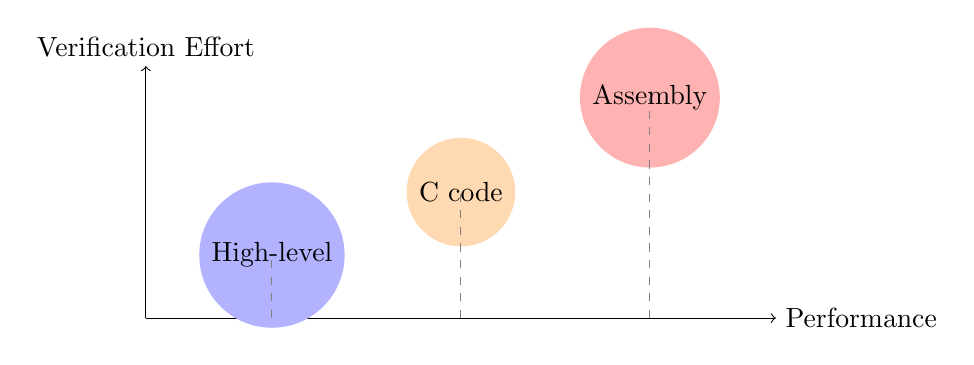
\begin{tikzpicture}[scale=0.8]
			\draw[->] (0,0) -- (10,0) node[right] {Performance};
			\draw[->] (0,0) -- (0,4) node[above] {Verification Effort};

			\node[circle,fill=blue!30] at (2,1) {High-level};
			\node[circle,fill=orange!30] at (5,2) {C code};
			\node[circle,fill=red!30] at (8,3.5) {Assembly};

			\draw[dashed,gray] (2,0) -- (2,1);
			\draw[dashed,gray] (5,0) -- (5,2);
			\draw[dashed,gray] (8,0) -- (8,3.5);
		\end{tikzpicture}
	\end{center}
\end{frame}

\begin{frame}{Looking ahead}
	\begin{center}
		\Large
		Verified crypto is becoming the new normal
	\end{center}
	\vspace{0.5em}
	\textbf{What we've achieved:}
	\begin{itemize}
		\item Performance parity with unverified code
		\item Real-world deployment at scale
		\item Growing ecosystem of tools
	\end{itemize}
	\vspace{0.5em}
	\textbf{What's next:}
	\begin{itemize}
		\item Better automation
		\item Shared infrastructure
		\item More platforms
		\item Broader adoption
	\end{itemize}
\end{frame}

\section{Implementation-Level Security}

\begin{frame}{The gap between theory and practice}
	\begin{center}
		\Large
		Design-level security is not enough!
	\end{center}
	\vspace{1em}
	\textbf{What we assume at design level:}
	\begin{itemize}
		\item Attackers choose inputs
		\item Attackers observe outputs
		\item That's it!
	\end{itemize}
	\vspace{0.5em}
	\textbf{Reality:}
	\begin{itemize}
		\item Attackers see much more
		\item Implementation details leak information
		\item Side-channels everywhere
	\end{itemize}
\end{frame}

\begin{frame}{Side channels: The hidden attack surface}
	\begin{center}
		\Large
		What are side channels?
	\end{center}
	\vspace{1em}
	\textbf{Information leaks through:}
	\begin{itemize}
		\item \textbf{Timing}: How long operations take
		\item \textbf{Memory access}: Which addresses are accessed
		\item \textbf{Power consumption}: How much energy is used
		\item \textbf{Electromagnetic radiation}: EM emissions
		\item \textbf{Acoustic}: Sound of computation
	\end{itemize}
	\vspace{0.5em}
	\begin{center}
		\textit{These are side-effects of computation, not intended outputs}
	\end{center}
\end{frame}

\begin{frame}{The devastating impact}
	\begin{center}
		\Large
		Side channels aren't just theoretical!
	\end{center}
	\vspace{1em}
	\textbf{Real attacks on real systems:}
	\begin{itemize}
		\item \textbf{RSA key recovery}: Full private keys extracted
		\item \textbf{AES key recovery}: Secret keys leaked
		\item \textbf{TLS attacks}: Lucky 13, Lucky Microseconds
		\item \textbf{Cloud attacks}: Cross-VM key extraction
	\end{itemize}
	\vspace{1em}
	\begin{center}
		\textit{Even ``secure'' algorithms become vulnerable in practice}
	\end{center}
\end{frame}

\begin{frame}{The constant-time solution}
	\begin{center}
		\Large
		Make execution independent of secrets
	\end{center}
	\vspace{1em}
	\textbf{Constant-time coding guidelines:}
	\begin{itemize}
		\item No secret-dependent branches
		\item No secret-dependent memory access
		\item No variable-time operations on secrets
		\item Same number of operations regardless of secret values
	\end{itemize}
	\vspace{0.5em}
	\begin{center}
		\textit{Note: ``Constant-time'' is about logical flow, not wall-clock time!}
	\end{center}
\end{frame}

\begin{frame}{Why constant-time is hard}
	\begin{center}
		\Large
		Natural code patterns become forbidden
	\end{center}
	\begin{columns}[t]
		\begin{column}{0.5\textwidth}
			\textbf{You can't write:}
			\begin{enumerate}
				\item \texttt{if (secret\_bit) \{ ... \}}
				\item \texttt{array[secret\_index]}
				\item Return early \texttt{if secret $\stackrel{?}{=}$ 0}
				\item Use division only when \texttt{secret != 0}\footnote{\url{https://kyberslash.cr.yp.to}}
			\end{enumerate}
		\end{column}
		\begin{column}{0.5\textwidth}
			\textbf{Instead, you must:}
			\begin{itemize}
				\item Use bit manipulation tricks
				\item Process all data uniformly
				\item Avoid natural optimizations
			\end{itemize}
		\end{column}
	\end{columns}
\end{frame}

\begin{frame}{Example: Constant-time selection}
	\textbf{Insecure (natural) code:}
	\begin{flushleft}
		\texttt{if (secret\_bit) \{}\\
		\texttt{~~~~result = a;}\\
		\texttt{\} else \{}\\
		\texttt{~~~~result = b;}\\
		\texttt{\}}
	\end{flushleft}
	\vspace{0.5em}
	\textbf{Secure (constant-time) code:}
	\begin{flushleft}
		\texttt{mask = -secret\_bit;~~// 0x00...0 or 0xFF...F}\\
		\texttt{result = (a \& mask) | (b \& \textasciitilde mask);}
	\end{flushleft}
	\vspace{0.5em}
	\begin{center}
		\textit{Same result, no branches, harder to understand!}
	\end{center}
\end{frame}

\begin{frame}{The compiler: Friend or foe?}
	\begin{center}
		\Large
		Your carefully written constant-time code\ldots

		\vspace{0.5em}

		...may not survive compilation!
	\end{center}
	\vspace{1em}
	\textbf{Compiler ``optimizations'' can:}
	\begin{itemize}
		\item Reintroduce branches
		\item Use lookup tables
		\item Short-circuit operations
		\item Use variable-time instructions
	\end{itemize}
	\vspace{0.5em}
	\begin{center}
		\textit{The compiler doesn't know about your security requirements}
	\end{center}
\end{frame}

\begin{frame}{Hardware betrays you too}
	\begin{center}
		\Large
		Even perfect assembly isn't safe
	\end{center}
	\vspace{1em}
	\textbf{Modern CPUs ``optimize'' behind your back:}
	\begin{itemize}
		\item Branch prediction
		\item Speculative execution
		\item Cache hierarchies
		\item Variable-latency instructions
	\end{itemize}
	\vspace{0.5em}
	\textbf{Result:}
	\begin{itemize}
		\item Timing variations you can't control
		\item Spectre/Meltdown-style attacks
		\item Cache timing attacks
	\end{itemize}
\end{frame}

\begin{frame}{Current practice: Hope and prayer}
	\begin{center}
		\Large
		How do we check constant-time today?
	\end{center}
	\vspace{1em}
	\textbf{1. Manual auditing}
	\begin{itemize}
		\item Expensive
		\item Time-consuming
		\item Error-prone
		\item Doesn't scale
	\end{itemize}
	\vspace{0.5em}
	\textbf{2. Testing wall-clock time}
	\begin{itemize}
		\item Fundamentally flawed approach
		\item Misunderstands constant-time
		\item Can't test all inputs
		\item Misses subtle leaks
	\end{itemize}
\end{frame}

\begin{frame}{A history of patches creating vulnerabilities}
	\begin{center}
		\Large
		Even experts get it wrong
	\end{center}
	\vspace{1em}
	\textbf{The vicious cycle in TLS:}
	\begin{enumerate}
		\item Original TLS timing vulnerability discovered
		\item Developers create a patch to fix it
		\item The patch itself is flawed
		\item This creates the Lucky 13 vulnerability
		\item Lucky 13 gets patched
		\item The Lucky 13 patch introduces a new timing vulnerability!
	\end{enumerate}
	\vspace{1em}
	\begin{center}
		\textit{Each ``fix'' introduced new vulnerabilities!}
	\end{center}
\end{frame}

\begin{frame}{The assembly escape hatch}
	\begin{center}
		\Large
		Can't trust the compiler? Skip it!
	\end{center}
	\vspace{1em}
	\textbf{Current practice:}
	\begin{itemize}
		\item Write critical code in assembly
		\item Implement constant-time directly
		\item Control every instruction
	\end{itemize}
	\vspace{0.5em}
	\textbf{The cost:}
	\begin{itemize}
		\item Platform-specific implementations
		\item Harder to audit
		\item More error-prone
		\item Maintenance nightmare
	\end{itemize}
\end{frame}

\begin{frame}{Enter computer-aided cryptography}
	\begin{center}
		\Large
		What if we could \textbf{prove} constant-time?
	\end{center}
	\vspace{1em}
	\textbf{CAC tools can:}
	\begin{itemize}
		\item Automatically check constant-time compliance
		\item Find subtle violations
		\item Even repair non-compliant code!
		\item Provide formal guarantees
	\end{itemize}
	\vspace{0.5em}
	\begin{center}
		\textit{Turn informal best practices into verified properties}
	\end{center}
\end{frame}

\begin{frame}{Formal leakage models}
	\begin{center}
		\Large
		What exactly does the attacker see?
	\end{center}
	\vspace{1em}
	\textbf{We must formally model leakage:}
	\begin{itemize}
		\item Define what operations leak
		\item Specify what information is revealed
		\item Abstract real-world observations
	\end{itemize}
	\vspace{0.5em}
	\textbf{Key insight:}
	\begin{center}
		\textit{Security = Leakage independent of secrets}
	\end{center}
	\vspace{0.5em}
	This is \textbf{observational non-interference}
\end{frame}

\begin{frame}{Hierarchy of leakage models}
	\begin{center}
		\Large
		Different models for different threats
	\end{center}
	\vspace{1em}
	\textbf{1. Program counter (PC) model}
	\begin{itemize}
		\item Leaks: Control flow only
		\item Protects against: Simple timing attacks
	\end{itemize}
	\vspace{0.5em}
	\textbf{2. Constant-time model}
	\begin{itemize}
		\item Leaks: PC + memory addresses
		\item Protects against: Cache attacks, timing attacks
		\item Most common in practice
	\end{itemize}
	\vspace{0.5em}
	\textbf{3. Size-respecting model}
	\begin{itemize}
		\item Leaks: PC + memory + operand sizes
		\item Protects against: Variable-time operations
	\end{itemize}
\end{frame}

\begin{frame}{Program counter leakage}
	\begin{center}
		\Large
		The simplest model: Control flow leaks
	\end{center}
	\vspace{1em}
	\textbf{What leaks:}
	\begin{itemize}
		\item Which branch was taken
		\item How many loop iterations
		\item Which functions were called
	\end{itemize}
	\vspace{0.5em}
	\textbf{Example violation:}
	\begin{flushleft}
		\texttt{if (password[i] != input[i]) \{}\\
		\texttt{~~~~return FAIL;~~// Early exit leaks position}\\
		\texttt{\}}
	\end{flushleft}
	\vspace{0.5em}
	\begin{center}
		\textit{Timing reveals where passwords differ!}
	\end{center}
\end{frame}

\begin{frame}{Constant-time leakage}
	\begin{center}
		\Large
		The standard model: PC + memory access
	\end{center}
	\vspace{1em}
	\textbf{Additionally leaks:}
	\begin{itemize}
		\item Which memory addresses are accessed
		\item Not the values, just the addresses!
	\end{itemize}
	\vspace{0.5em}
	\textbf{Example violation:} \texttt{result = lookup\_table[secret\_index]}
	\vspace{0.5em}
	\begin{center}
		\textit{Cache attacks can recover \texttt{secret\_index}}
	\end{center}
\end{frame}

\begin{frame}{The verification promise}
	\begin{center}
		\Large
		Prove once, secure forever
	\end{center}
	\vspace{1em}
	\textbf{Verification tools can prove:}
	\begin{itemize}
		\item Code follows constant-time discipline
		\item For all possible secret values
		\item Through all execution paths
		\item Despite complex control flow
	\end{itemize}
	\vspace{0.5em}
	\begin{center}
		\textit{No more hoping your tests caught everything}
	\end{center}
\end{frame}

\begin{frame}{The fine print}
	\begin{center}
		\Large
		What are we actually proving?
	\end{center}
	\vspace{1em}
	\textbf{Important caveats:}
	\begin{itemize}
		\item Proofs are relative to the leakage model
		\item Hardware may leak more than modeled
		\item New attacks may require new models
		\item Speculative execution is particularly tricky
	\end{itemize}
	\vspace{0.5em}
	\begin{center}
		\textit{We prove security in our model, not absolute security}
	\end{center}
\end{frame}

\begin{frame}{The gap remains}
	\begin{center}
		\Large
		From verified code to secure execution
	\end{center}
	\vspace{1em}
	\textbf{Remaining challenges:}
	\begin{itemize}
		\item Compiler may still break guarantees
		\item Hardware may not respect assumptions
		\item Micro-architectural attacks (Spectre/Meltdown)
		\item Physical side channels
	\end{itemize}
	\vspace{0.5em}
	\textbf{Partial solutions:}
	\begin{itemize}
		\item Verify at assembly level
		\item Use verified compilers
		\item Hardware/software co-design
	\end{itemize}
\end{frame}

\begin{frame}{Looking forward}
	\begin{center}
		\Large
		Implementation security is an arms race
	\end{center}
	\vspace{1em}
	\textbf{The cycle continues:}
	\begin{enumerate}
		\item New side channels discovered
		\item Update leakage models
		\item Develop countermeasures
		\item Verify implementations
		\item Repeat\ldots
	\end{enumerate}
	\vspace{0.5em}
	\begin{center}
		\textit{CAC tools help us stay ahead in this race}
	\end{center}
\end{frame}

\begin{frame}{Computational analysis tools overview}
	\bigimagewithcaption{verif-implementations.png}{Source: Manuel Barbosa, Gilles Barthe, Karthikeyan Bhargavan, Bruno Blanchet, Cas Cremers, Kevin Liao and Bryan Parno, SoK: Computer-Aided Cryptography, IEEE Symposium on Security and Privacy, 2021.}
\end{frame}

\section{Case Study: Lessons Learned from TLS}

\begin{frame}{Case Study: Transport Layer Security (TLS)}
	\begin{center}
		\Large
		One of the most important real-world deployments of cryptography
	\end{center}
	\vspace{1em}
	\begin{itemize}
		\item Powers HTTPS everywhere
		\item Secures email, VPNs, messaging
		\item Protects billions of connections daily
	\end{itemize}
	\vspace{1em}
	\begin{center}
		\textit{But the road to secure TLS was long and painful\ldots}
	\end{center}
\end{frame}

\begin{frame}{The dark ages: TLS before 1.3}
	\begin{center}
		\Large
		A reactive cycle of attacks and patches
	\end{center}
	\vspace{1em}
	\textbf{The endless loop:}
	\begin{enumerate}
		\item \textbf{Attack found} -- Security researchers discover vulnerability
		\item \textbf{Quick patch} -- Rushed fix deployed to stop bleeding
		\item \textbf{Long-term fix} -- More thoughtful solution developed
		\item \textbf{Next version} -- Protocol updated with fixes
		\item \textbf{Back to step 1} -- New attacks emerge on ``fixed'' version
	\end{enumerate}
	\vspace{0.5em}
	\begin{center}
		\textit{No substantial academic analysis during design}
	\end{center}
\end{frame}

\begin{frame}{Early academic analysis: Too simple}
	\begin{center}
		\Large
		Academics studied ``toy'' versions of TLS
	\end{center}
	\vspace{1em}
	\textbf{Why oversimplified models?}
	\begin{itemize}
		\item Full protocol too complex
		\item Analysis tools couldn't handle it
		\item Focused on cryptographic core only
	\end{itemize}
	\vspace{0.5em}
	\textbf{The consequence:}
	\begin{itemize}
		\item Missed many real attacks
		\item False sense of security
		\item Gap between theory and practice
	\end{itemize}
\end{frame}

\begin{frame}{The complexity explosion}
	\begin{center}
		\Large
		When academics looked at \textit{real} TLS\ldots
	\end{center}
	\vspace{1em}
	\begin{center}
		\textbf{Many new attacks discovered!}
	\end{center}
	\vspace{0.5em}
	\begin{itemize}
		\item BEAST
		\item CRIME
		\item Lucky 13
		\item POODLE
		\item Logjam
		\item And many more, as discussed in our TLS session!
	\end{itemize}
	\vspace{0.5em}
	\begin{center}
		\textit{The devil was in the details we'd been ignoring}
	\end{center}
\end{frame}

\begin{frame}{TLS 1.3: A paradigm shift}
	\begin{center}
		\Large
		From reactive patching to proactive design
	\end{center}
	\vspace{1em}
	\textbf{Revolutionary changes:}
	\begin{itemize}
		\item Academic community consulted \textbf{during} design
		\item Multiple drafts analyzed formally
		\item 28 drafts over 4+ years!
		\item Unprecedented collaboration
	\end{itemize}
	\vspace{0.5em}
	\begin{center}
		\textit{First major protocol designed with formal analysis in mind}
	\end{center}
\end{frame}

\begin{frame}{Computer-aided cryptography joins the party}
	\begin{center}
		\Large
		Multiple tools, multiple approaches
	\end{center}
	\vspace{1em}
	\textbf{Verified implementations:}
	\begin{itemize}
		\item Implementations with cryptographic proofs
	\end{itemize}
	\vspace{0.5em}
	\textbf{Symbolic analysis:}
	\begin{itemize}
		\item ProVerif models
		\item Tamarin models
	\end{itemize}
	\vspace{0.5em}
	\textbf{Computational analysis:}
	\begin{itemize}
		\item CryptoVerif proofs
	\end{itemize}
	\vspace{0.5em}
	\begin{center}
		\textit{A comprehensive assault on insecurity!}
	\end{center}
\end{frame}

\begin{frame}{Lesson 1: Formal methods find real flaws}
	\begin{center}
		\Large
		The process of formally specifying reveals bugs
	\end{center}
	\vspace{1em}
	\textbf{Just trying to write formal specs uncovers issues:}
	\begin{itemize}
		\item Ambiguities in the standard
		\item Implicit assumptions
		\item Corner cases
		\item Unclear security goals
	\end{itemize}
	\vspace{0.5em}
	\begin{center}
		\textit{If you can't specify it clearly, it's probably broken}
	\end{center}
\end{frame}

\begin{frame}{Real attacks found by formal analysis}
	\begin{center}
		\Large
		These aren't theoretical problems!
	\end{center}
	\vspace{1em}
	\textbf{TLS 1.2 analysis (Bhargavan et al.):}
	\begin{itemize}
		\item Alert fragmentation attacks
		\item Fingerprinting attacks
		\item Led to Triple Handshake attack discovery
	\end{itemize}
	\vspace{0.5em}
	\textbf{TLS 1.3 draft 10 (Cremers et al.):}
	\begin{itemize}
		\item Client impersonation in PSK-resumption
		\item Fixed in draft 11
	\end{itemize}
\end{frame}

\begin{frame}{More attacks from formal analysis}
	\textbf{TLS 1.3 draft 13 (Bhargavan et al.):}
	\begin{itemize}
		\item New attack on 0-RTT client authentication
		\item ProVerif found what humans missed
	\end{itemize}
	\vspace{0.5em}
	\textbf{TLS 1.3 draft 21 (Cremers et al.):}
	\begin{itemize}
		\item Unexpected behavior affecting authentication
		\item Tamarin revealed subtle issues
	\end{itemize}
	\vspace{1em}
	\begin{center}
		\Large
		Nearly all discoveries led to protocol improvements!
	\end{center}
\end{frame}

\begin{frame}{Lesson 2: Protocols are moving targets}
	\begin{center}
		\Large
		28 drafts = 28 different protocols!
	\end{center}
	\vspace{1em}
	\textbf{The challenge:}
	\begin{itemize}
		\item Significant changes between drafts
		\item Previous analyses quickly outdated
		\item Manual proofs become stale
		\item Months of work invalidated
	\end{itemize}
	\vspace{0.5em}
	\begin{center}
		\textit{How do you hit a moving target?}
	\end{center}
\end{frame}

\begin{frame}{Machine-checked proofs to the rescue}
	\begin{center}
		\Large
		Automated tools can evolve with the protocol
	\end{center}
	\vspace{1em}
	\textbf{Key advantages:}
	\begin{itemize}
		\item Update models incrementally
		\item Re-run verification automatically
		\item Catch regressions immediately
		\item Ensure fixes don't break other properties
	\end{itemize}
	\vspace{0.5em}
	\textbf{Manual proofs can't compete:}
	\begin{itemize}
		\item Too slow to update
		\item Error-prone modifications
		\item Can't keep pace with drafts
	\end{itemize}
\end{frame}

\begin{frame}{Lesson 3: Design for verifiability}
	\begin{center}
		\Large
		Small changes can dramatically simplify analysis
	\end{center}
	\vspace{1em}
	\textbf{TLS 1.3 embraced verification-friendly changes:}
	\begin{itemize}
		\item Better key separation in key schedule
		\item Consistent message tagging
		\item More transcript information in exchanges
		\item Cleaner state machine
	\end{itemize}
	\vspace{0.5em}
	\begin{center}
		\textit{Negligible performance impact, huge verification benefit}
	\end{center}
\end{frame}

\begin{frame}{Examples of verification-friendly changes}
	\textbf{Key separation:}
	\begin{itemize}
		\item Different keys for different purposes
		\item Enables modular security proofs
		\item Prevents cross-protocol attacks
	\end{itemize}
	\vspace{0.5em}
	\textbf{Consistent tagging:}
	\begin{itemize}
		\item Every message type clearly labeled
		\item No ambiguity in parsing
		\item Simplifies formal models
	\end{itemize}
	\vspace{0.5em}
	\textbf{Transcript inclusion:}
	\begin{itemize}
		\item Include history in handshake messages
		\item Makes consistency proofs easier
		\item Prevents replay attacks
	\end{itemize}
\end{frame}

\begin{frame}{The impact: A new standard for standards}
	\begin{center}
		\Large
		TLS 1.3 changed how protocols should be designed
	\end{center}
	\vspace{1em}
	\textbf{The new playbook:}
	\begin{enumerate}
		\item Involve formal methods experts early
		\item Design with verification in mind
		\item Use tools throughout development
		\item Update proofs with each draft
		\item Fix issues before standardization
	\end{enumerate}
	\vspace{0.5em}
	\begin{center}
		\textit{From ``ship and patch'' to ``verify and ship''}
	\end{center}
\end{frame}

\begin{frame}{Why this matters beyond TLS}
	\begin{center}
		\Large
		TLS 1.3 proved formal methods can scale
	\end{center}
	\vspace{1em}
	\textbf{Key achievements:}
	\begin{itemize}
		\item Analyzed a \textit{real} protocol, not a toy
		\item Found and fixed \textit{real} vulnerabilities
		\item Kept pace with \textit{real} development
		\item Influenced \textit{real} design decisions
	\end{itemize}
	\vspace{0.5em}
	\begin{center}
		\textit{This is the future of secure protocol design}
	\end{center}
\end{frame}

\begin{frame}[plain]
	\titlepage
\end{frame}
\end{document}
